
\documentclass[./thesis.tex]{subfiles}

 
\begin{document}


\section{Principle of matrix dressing}

So far we have used the second order perturbation to build a zeroth-order wavefunction $\ket \Psi$ using CISPI, and estimate its distance to the FCI energy with a stochastic estimation of $\EPT$.

In both cases we have computed the interaction between $\ket \Psi$ and the external space, but we have not let $\ket \Psi$ be revised under those interactions. This idea is based on the so-called \Bk approximation proposed by Gershgorn and Shavitt.\cite{Gershgorn_1968}

This can be achieved using the intermediate Hamiltonian theory,\cite{0305-4470-18-5-014} intermediate Hamiltonians being a class of effective Hamiltonians\cite{lindgren1982atomic} where not all roots are exact eigenvalues of the full Hamiltonian.
The principle is to build a so-called intermediate Hamiltonian ${\bf \tilde H}$ which, when diagonalized, yields a wavefunction that takes into account the effect of an external space on the internal space. 


Sticking to the state-specific case, the general principle can be understood as follows. This formulation, as it is limited to the state-specific case, is somewhat different and wishes to be more intuitive than the one presented in the article presented in section~\ref{sec:matrix_article}.
Fully taking into account the external space requires to solve 

\newcommand{\Hzero}{{H}^{(0)}}
\newcommand{\hcplbold}{{\bf h}}
\newcommand{\Hzerobold}{{\bf H}^{(0)}}
\newcommand{\hcpl}{{h}}

\begin{equation}
\begin{pmatrix}
\Hzerobold &  \hcplbold\\ 
\hcplbold^\dagger & {\bf H}^{(1)}
\end{pmatrix} \begin{pmatrix}
{\bf c}\\ 
{\bf c}^\alpha
\end{pmatrix}=E\begin{pmatrix}
{\bf c}\\ 
{\bf c}^\alpha
\end{pmatrix}
\end{equation}
with ${\bf H}^{(0)}$ and ${\bf H}^{(1)}$ the zeroth and first-order Hamiltonians, $\bf h$ the coupling term between zeroth and first order spaces, ${\bf c}$ the coefficients for the zeroth-order space and ${\bf c}^\alpha$ the coefficients for the external space.

This diagonalization is normally not feasible due to the external space being too large. However, if we are willing to neglect the external-to-external and internal-to-external influences ---~in other words, if we freeze the external space~--- we can only solve the eigenequations associated with internal determinants. As usual, associating $I$ and $J$ to internal determinants and $\alpha$ to external ones, for line $I$ we have
\begin{equation}
\qty(\Hzero_{II} - E)c_I  + \sum_{J \neq I} {c_J \Hzero_{IJ}} + \sum_\alpha {c_\alpha \hcpl_{I \alpha}} = 0.
\label{eq:eignen_sum}
\end{equation}

Obviously, since we froze the external space, we need some way to estimate ${\bf c}^\alpha$. In the presented paper, we used a perturbative estimation consistently with what we used in CIPSI and $\EPT$. Because of this, whenever $\bf c$ is revised, ${\bf c}^\alpha$ needs to be recomputed as well. This makes \Bk an iterative method.

Because the $c_\alpha$ coefficients are frozen, $\sum_\alpha {c_\alpha H_{I \alpha}}$ is merely a constant added to the eigenequation of line $I$. Renaming this term $\delta_I$, we can rewrite Eq.\eqref{eq:eignen_sum} as
\begin{equation}
\qty(\Hzero_{II} - E + \frac{\delta_I}{c_I})c_I  + \sum_{J \neq I} {c_J \Hzero_{IJ}} = 0.
\label{eq:eignen_delta}
\end{equation}
It appears solving this new system of linear equations is equivalent to diagonalizing 
\begin{equation}
{\bf \tilde H} = \Hzerobold + \Deltabold 
\end{equation}
with $\Deltabold$ a diagonal matrix
\begin{equation}
\begin{cases}
\Delta_{II}=\frac{\delta_I}{c_I}\\
\Delta_{IJ}=0 & \text{if } I \neq J.
\end{cases}
\end{equation}

Here ${\bf \tilde H}$ is the intermediate Hamiltonian and ${\bf \Delta}$ the so-called \emph{dressing matrix}. Consequently ${\bf \tilde H}$ may be referred to as a \emph{dressed Hamiltonian}. 
Note that the dressing matrix is diagonal because of an arbitrary rewriting of Eq.~\eqref{eq:eignen_sum} into Eq.~\eqref{eq:eignen_delta}. We can actually build ${\bf \Delta}$ in any way that fulfills
\begin{equation}
\sum_J c_J \Delta_{IJ}  = \delta_I.
\label{eq:arbitrary_dressing}
\end{equation}

While the choice of which elements of $\Deltabold$ are non-zero is arbitrary, it can be of importance for numerical reasons (in addition to obvious storage reasons). However, because we diagonalize ${\bf \tilde H}$ using a Davidson diagonalization, this is of no concern to us. Indeed, Davidson's diagonalization only requires the knowledge of ${\bf \tilde H} {\bf c}$ and of the diagonal of ${\bf \tilde H}$ 
\begin{equation}
{\bf \tilde H} {\bf c} = \Hzerobold\, {\bf c} + {\bf \Delta}\, {\bf c}.
\end{equation}
Because of Eq.~\eqref{eq:arbitrary_dressing}, we have by construction
\begin{equation}
\Deltabold\, {\bf c} = {\pmb \delta}
\end{equation}
with ${\pmb \delta}$ the vector $\qty(\delta_1, \ldots, \delta_{\Ndet})$.
Algorithmically, it boils down to computing ${\pmb \delta}$, which is more expensive to compute than the product ${\bf \tilde H}\,{\bf U}$ needed for Davidson's diagonalization. But unlike ${\bf \tilde H}\,{\bf U}$ which is too large to be stored, and needs to be re-computed on the fly at each Davidson iteration, ${\pmb \delta}$ is fixed and can easily be stored.


An improved version to this original idea was proposed by Davidson and co-workers under the name shifted-\Bk,\cite{Nitzsche_1978a, Nitzsche_1978b, Rawlings_1983, Kozlowski_1995, Kozlowski_1994a, Kozlowski_1994b, Kozlowski_1994c} which is the one we implemented. Details about this improvement and on how it can be generalized to a multi-state case are available in the presented article (section~\ref{sec:matrix_article}).



\section{Implementation}

\subsection{From $\EPT$ to matrix dressing}

In some respect, computing the dressing matrix is akin to computing $\EPT$. The dressing matrix can be decomposed as a sum of elementary dressing matrices $\deltabold_\alpha$, each one associated with a particular $\ket \alpha$, just like $\EPT$ is a sum of $e_\alpha$. It is possible to pack those elementary matrices together like we packed $\ket \alpha$ together for $\EPT$.
\begin{equation}
\deltabold_I = \sum_{\alpha \in \mathcal{A}_I} \deltabold_\alpha
\end{equation}
\begin{equation}
\deltabold = \sum_{I} \deltabold_I
\end{equation}
So as we only need $\tilde{\bf H}{\bf c}$ for Davidson's algorithm, the quantity we sample is 
\begin{equation}
\deltabold_I = \Deltabold_I\, {\bf c} = \sum_{\alpha \in \mathcal{A}_I} \deltabold_\alpha\, {\bf c}
\end{equation}

Thus, ${\pmb \delta}_I$ is a sum over external determinants, and requires to find connections between those determinants and the wavefunction. Presumably, the elementary dressing vectors $\deltabold_I$ will have a norm decreasing like $e_I$. Indeed, 
\begin{equation}
e_I = \frac{{\bf c}^\dagger\, \Deltabold_I\, {\bf c}}{{\bf c}^\dagger {\bf c}} = {\bf c}^\dagger \deltabold_I
\label{eq:c_delta_i}
\end{equation}
Using the Cauchy–Schwarz inequality
\begin{equation}
e_I \le \sqrt{ \qty (\deltabold_I^\dagger \deltabold_I) \qty({\bf c}^\dagger {\bf c}) } \le
\norm{\deltabold_I}.
\end{equation}

With that in mind, is seems possible, theoretically, to generalize our hybrid stochastic-deterministic PT2 for computing dressing vectors.
However there are a few significant differences.
\begin{itemize}
\item
We were estimating a scalar, now we are estimating a vector. How can we quickly estimate the running error?
To address this problem, we decided to compute the statistical error associated with $E_{\Delta}$, the energy contribution of $\Deltabold$. Our dressed matrix being $\mathbf{H} + \Deltabold$, the energy is
\begin{equation}
\frac{\mel{\Psi}{\widehat{H} + \widehat{\Delta}}{\Psi}}{\braket{\Psi}{\Psi}} =
\frac{ \Hij{\Psi}{\Psi}}{\braket{\Psi}{\Psi}} + \frac{\mel{\Psi}{\widehat{\Delta}}{\Psi}}{\braket{\Psi}{\Psi}} = \Evar + E_{\Delta} 
\end{equation}
where $E_{\Delta}$ is estimated the same way as $\EPT$ was, based on individual contributions $e_I$ (see eq.~\eqref{eq:c_delta_i}).
\item
In both cases we have $\Ngen$ samples, however in the case of $\EPT$ each sample is a scalar, here each sample is a vector of size $\Ndet$. It is easy to store $\Ngen$ scalars, not to store $\Ngen$ vectors of size $\Ndet$. In addition, these vectors must be transmitted from slave nodes to a master node, creating a potential network bottleneck, scaling with $\Ndet$.
\item
In the case of $\EPT$, each connection found only requires an increment of some elements of $P(G_{pq})$. At no point two connections need to be known at the same time. This is different for methods implemented with matrix dressing. It is possible that one needs to know the detail of which internal determinants an $\ket \alpha$ connects to, in order to be able to compute $\deltabold_\alpha$.
\end{itemize}



Implementationally speaking, just like the state-specific version requires computing a single $\deltabold$ vector, the multi-state version requires a $\deltabold^{(k)}$ vector to be computed for each desired state $k$. This, in principle, should come with minimal cost, since the loop over states can be set as the innermost one. 

In practice, since the exact computation of $\deltabold^{(k)}$ is as expensive than that of $\EPT$, we need to use the same hybrid stochastic-deterministic approach. Unfortunately, using state-average coefficients for the sampling did not yield satisfying results, so we have to stick to state-specific sampling and thus compute each $\deltabold^{(k)}$ individually. Therefore we will ignore the state from now on.
The multi-state Davidson diagonalization, however, is done a single time per shifted-\Bk iteration.

\subsection{Reduction of the memory bottleneck}

The core idea to reduce the required storage is that, in a Monte-Carlo scheme, even an ``exotic'' one like our hybrid approach, the estimated result has to be a linear combination of all samples. At any point $m$ of the Monte-Carlo computation corresponding to $M_m$ combs having been drawn, we can write our estimated dressing vector $\deltabold^m$ as :


\begin{equation}
\deltabold^m = \sum_{I=1}^{\Ngen} \mu^m_{I} \deltabold_I
\end{equation}


The values for $\mu^m_I$ have no dependence on those of $\deltabold_I$. They only depend on what samples have been drawn so far. Since we decide beforehand which combs are going to be drawn, we can compute the ${\pmb \mu}$ vector for any point of the Monte-Carlo before any sample has been computed. The values we chose for $M_m$ act as predetermined \emph{checkpoints}.

\begin{comment}
\begin{figure}[h!]
	\begin{center}
		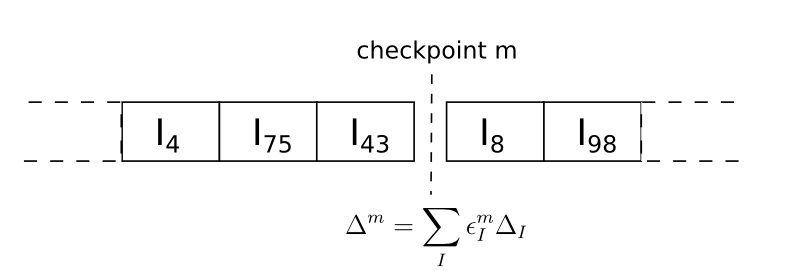
\includegraphics[width=1.00\columnwidth]{figures/matrix_dressing/checkpoint}
		\caption{\label{checkpoint}}
		A REFAIRE EN VERTICAL AVEC Q[j]
	\end{center}
\end{figure}
\end{comment}


They can be set at any arbitrary point, but they must be determined beforehand and cannot be changed during the computation ; we will only be able to get results at those points.
For checkpoint $m$, we start with a zero-initialized vector for $\deltabold^m$, and
we increment it each time an elementary vector $\deltabold_I$ is computed:
\begin{equation}
\deltabold^m \gets \deltabold^m + \mu_I^{m} \deltabold_I.
\end{equation}
Once this has been done, $\deltabold_I$ can be discarded. Indeed, when checkpoint $m$ is reached, $\deltabold^{m}$ has its final value, as obviously $\mu_I^{m} = 0$ for any $\deltabold_I$ sample that hasn't yet been drawn at checkpoint $m$.
For convenience, some parameters can be defined as functions of a checkpoint reached:
$\dot t_m$, the first non-deterministic tooth when checkpoint $m$ is reached, and
\begin{equation}
\dot n_0(m) = n_0(\dot t_m),
\end{equation}
the size of the deterministic range when $m$ is reached.
$\mu^m_I$ is defined as follows
\begin{equation}
\mu^m_I = 
\begin{cases}
1 & \text{if } i \leq \dot n_0(m) \\
\frac{W_T \times M_{m,I}}{w_I \times M_m} & \text{if } I > \dot n_0(m)
\end{cases}
\end{equation}
with $M_{m,I}$ the number of times generator $I$ has been drawn at checkpoint $m$.


The memory cost for a checkpoint $m$ is $2 \times \Ndet$ floats, corresponding to the storage of ${\pmb \mu}^m$ and $\deltabold^m$. This cost is small enough to allow setting up quite a few checkpoints. However, in addition to this memory cost, comes some computational cost. If we set up $\Ncp$ checkpoints, it implies each time a sample is drawn, we will have, theoretically, to increment $\Ncp$ vectors of size $\Ndet$. For quicker tasks, this price may not be negligible. It gets worse if, as was the case in our first implementation, a collector is in charge of updating checkpoints for multiple slaves. 

We can drastically reduce the amount of writing required for each sample by rewriting $\deltabold^m$.
First, we define $\deltabold^{D,t}$ as the total dressing contribution for tooth $\mathcal{T}_t$
\begin{equation}
\deltabold^{D,t} = \sum_{I \in \mathcal{T}_t} \deltabold_I.
\end{equation}
We rewrite $\deltabold^m$ as
\begin{equation}
\label{eq:rewrite1}
\deltabold^{m} = \sum_{t=0}^{\dot t_m - 1} \deltabold^{D,t}+ \frac{1}{M_m} \sum_{I} \gamma^m_{I} \deltabold_I.
\end{equation}
The second term being $\deltabold^m$ without its deterministic contribution, we can trivially write, defining $\gamma^ 0_I=0$ for convenience,
\begin{equation}
\gamma^m_I = 
\begin{cases}
0 & \text{if } I \leq \dot n_0(m) \vee m=0 \\
\mu^m_I \times M_m = \frac{W_T \times M_{m,I}}{w_I} & \text{if } I > \dot n_0(m) \wedge m \neq 0
\end{cases}.
\end{equation}
We define
\begin{align}
\deltabold^{S,m} = \sum_I (\gamma^m_I - \gamma^{m-1}_I) \deltabold_I,
\end{align}
we can rewrite the second term of Eq.~\eqref{eq:rewrite1}
\begin{equation}
\frac{1}{M_m}\sum_{I} \gamma^m_{I} \deltabold_I = \frac{1}{M_m} \sum_{p=1}^m \deltabold^{S,p}
\end{equation}
and write the final form or $\deltabold^m$ as
\begin{equation}
\deltabold^m=\sum_{t=0}^{\dot t_{m}-1} \deltabold^{D,t} + \frac{1}{M_m} \sum_{p=1}^m \deltabold^{S,p}.
\end{equation}

The vectors we need to store are $\deltabold^{D,t}$ and $\deltabold^{S,m}$. Each time we compute an elementary dressing vector $\deltabold_I$, the need for update goes as follows
\begin{itemize}
\item
$\deltabold^{D,t}$ with $I \in \mathcal{T}_t$. This is exactly one write.
\item
$\deltabold^{S,m}$ where $\gamma^m_I - \gamma^{m-1}_I \neq 0$. This is
 \begin{itemize}
 \item No write if generator $\ket{D_I}$ is moved to $\mathcal{D}$ in the same checkpoint it is first drawn or computed for tooth filling
 \item Otherwise, one write per checkpoint in which it is drawn until the one where it is moved to $\mathcal{D}$, inclusive.
 \end{itemize}
 While this increases the theoretical maximum of writes to $\Ncp+1$ per sample, it is much lower in practice.
\end{itemize}

For convenience we define
\begin{equation}
\tilde \mu^m_I = \gamma^m_I - \gamma^{m-1}_I.
\end{equation}
The task queue is built in a fashion similar to the one for the $\EPT$ computation, with some differences.
\begin{itemize}
\item
$M_{m,I}$ are evaluated for the computation of $\tilde \mu^m_I$.
\item
Instead of $R$ we evaluate $R^{-1}$, based on indices of checkpoints rather than of combs. In the algorithm for $\EPT$, when the first $j$ tasks are completed, the comb of index $R[j]$ is available. Here, when the first $R^{-1}[m]$ tasks have been completed, checkpoint $m$ has just become computable.
\item
We create sample subsets $\mathcal{P}_m$ associated with checkpoints. $I \in \mathcal{P}_m$ iff
\begin{equation}
R^{-1}[m-1] < j \leq R^{-1}[m]  \;; R^{-1}[0] = 0
\end{equation}
with $j$ the task index associated with $I$, i.e. $Q[j]=I$. These sets are tracked using an array $P$ so that $P[I]=m$ iff $I \in \mathcal{P}_m$.

\end{itemize}

\begin{figure}[h!]
	\begin{center}
		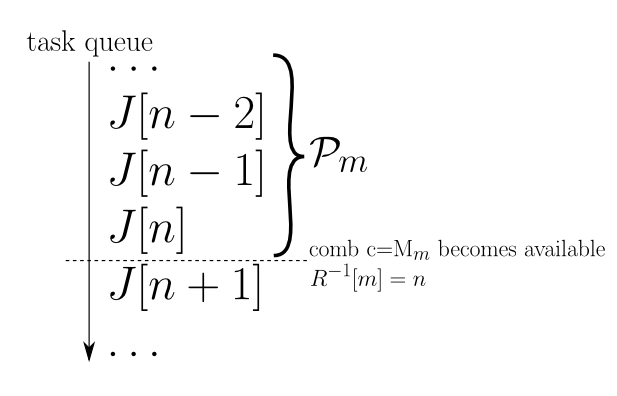
\includegraphics[width=0.45\columnwidth]{figures/matrix_dressing/taskqueue}
		\caption{Task queue divided in checkpoints $\mathcal{P}_m$. The task array $Q$ contains the indices of samples to be computed. When all tasks in sets $\mathcal{P}_{p\leq m}$ have been computed, checkpoint $m$ is computable.
}
		\label{fig:task_queue}
	\end{center}
\end{figure}

\begin{algorithm}
	\caption{Compute task queue and checkpoints.}
	\label{PRECOMPUTE_MONTECARLO}
		\KwData{$M_m$ the desired number of combs for checkpoints $m$. $M_0 = 0$ for convenience. $M_{n+1} > M_n$, $\exists M_n > \Ngen$}
		\KwResult{$Q$ the task array, $\Ncp$ the number of checkpoints, $P$ the array so that $P[I] = m$ iff $I \in \mathcal{P}_m$, $R^{-1}$ the array so that checkpoint $m$ becomes available when the first $R^{-1}[m]$ tasks have been computed.}
		$\tilde M$ array of size $\Ndet$ initialized with $0$\;
		$u$ array of size $\Ngen$ initialized with random numbers $\in [0,1)_\mathbb{R}$ \;
		$d$ a boolean array of size $\Ngen$ initialized with $\FALSE$.
		
		$R^{-1}[0] \gets 0$ \;
		$N_c \gets 0$ \;
		$N_Q \gets n_0(1)$ \;
		\For{$i\gets 1,N_Q$}{
			$d[i] \gets \TRUE$ \;
			$Q[i] \gets i$ \;
		}
		
		$\Ncp \gets 0$ \;
		$F \gets N_Q+1$ \;
		\While{$N_Q < \Ngen$}{
			ADD\_COMB shown as algorithm \ref{alg:FILL_TOOTH} \;
			FILL\_TOOTH shown as algorithm \ref{alg:ADD_COMB} \;
			\If{$M_{\Ncp+1} = N_c$}{
				$\Ncp \gets \Ncp+1$ \;
				$R^{-1}[\Ncp] \gets N_Q$ \;
				 %$cpthreshold[m] \gets N_Q$ \;
				$M_{\Ncp,*} \gets \tilde M$ \;
			} 
		}
		\If{$R^{-1}[\Ncp] \neq N_Q$}{
			\tcc{Adds a final checkpoint.}
			$\Ncp \gets \Ncp+1$ \;
			$R^{-1}[\Ncp] = N_Q$ \;
		}
		optimize task queue with algorithm \ref{alg:OPTIMIZE_MONTECARLO} \;
		\For{$m\gets 1,\Ncp$}{
		\For{$i\gets R^{-1}[m-1]+1,R^{-1}[m]$}{
			$P[Q[i]] \gets m$ \;
		}
		}
\end{algorithm}

%An extra array $P[i]=m$ is built, mapping a sample index $i$ to the checkpoint $m$ in which it is first needed ; in other words, when sample $i$ needs to be evalutated, checkpoints up to $m-1$ have been fully built.


\begin{algorithm}
	\KwResult{Modifies $Q$ the task array and $R^{-1}$ the array defining the boundaries of checkpoints in $Q$.}
	\caption{Optimize checkpoints so that they are available faster.}
	\label{alg:OPTIMIZE_MONTECARLO}
	
	%\SetKwFunction{FMain}{OPTIMIZE\_MONTECARLO}
	%\SetKwProg{Fn}{Function}{:}{}
	
	%\Fn(\tcc*[h]{Optional algorithm to reorder tasks so checkpoints are reached as fast as possible.}){\FMain{some args}}{
		%$lastNj \gets 1$ \;
		\For{$m\gets 1,\Ncp$}{
			$Nmoved \gets 0$ \;
			$firstTask \gets R^{-1}[m-1]+1$ \;
			\For{$j\gets firstTask,R^{-1}[m]$}{
				\If{$M_{m,Q[j]} = 0 \wedge Q[j] > \dot n_0(m)$}{
					\tcc{Ensures moved tasks are at the end of the checkpoint once sorted.}
					$Q[j] \gets Q[j] + \Ngen$ \;
					$Nmoved \gets Nmoved + 1$ \;
				}
			}
			Sort array $Q$ from $firstTask$ to $R^{-1}[m]$, inclusive \;
			\tcc{Moved tasks are sent to the next checkpoint.}
			$R^{-1}[m] \gets R^{-1}[m] - Nmoved$ \;
			\tcc{Restores the original values of moved tasks.}
			\For{$j\gets R^{-1}[m]+1,R^{-1}[m] + Nmoved$}{
				$Q[j] \gets Q[j] - \Ngen$ \;	
			}
		}
		%$k \gets 1$ \;		
		%\For{$i\gets 2,\Ncp$}{
	%		\If{$R^{-1}[k] \neq R^{-1}[i]$}{
	%			$k \gets k + 1$ \;	
%				$R^{-1}[k] \gets R^{-1}[i]$ \;
%			}		%
%		}
%		$\Ncp \gets k$ \;
\end{algorithm}

Algorithm~\ref{PRECOMPUTE_MONTECARLO} presents the computation of the task queue, and
algorithm \ref{alg:OPTIMIZE_MONTECARLO} is an optional reorganization of task order. It ensures results for a checkpoint are available as quickly as possible, without altering them.
%Some checkpoints may however be removed if no extra computation is required to reach the next one ; this situation can't happen in the unoptimized task queue, because of the tooth filling. Two things are taken into consideration:
\begin{itemize}
\item
Because no result is available between two checkpoints, the order in which tasks are processed between two checkpoints is irrelevant for the result. So, as is usually the case with parallel tasks, we would like to do the longest tasks first, so that we don't get a load imbalance due to a massive task being done last. Therefore, tasks should always be in ascending order (descending computational time) between two checkpoints.
\item
Because of the ``tooth filling'', sometimes samples computed inside a checkpoint are not involved in its result. Since tooth filling picks the first non-computed tasks, they tend to be of high computational cost. The algorithm iterates over checkpoints in ascending order, each time moving such a sample to the next checkpoint. Thus, every sample is moved to the first checkpoint it is actually involved in, either deterministically or stochastically.
\end{itemize}



\begin{algorithm}
	\caption{Computation of $\tilde \mu$, $\dot t$ and $\dot n_0$.}
	\label{COMPUTE_MU}
	\KwData{$Q$, $R^{-1}$, $n_0$, $\Nteeth$}
		\KwResult{ $\tilde \mu$, $\dot t$ and $\dot n_0$}
		$\tilde \mu^*_* \gets 0$ \;
		$F \gets n_0(1)+1$ \;		
		\For{$m\gets 1,\Ncp$}{
			\For{$i\gets R^{-1}[m-1]+1,R^{-1}[m]$}{
				$d[Q[i]] \gets true$ \;			
			}
			\While{$d(U+1)$}{
				$U \gets U+1$ \;
		  	}
		  	
		  	$\dot t_m \gets \Nteeth+1$ \;
			$\dot n_0(m) \gets \Ngen$ \;
			
			\For{$t\gets 2,\Nteeth+1$}{
				\If{$U < n_0(t)$}{% rTeethI[t]$}{
					$\dot t_m \gets t-1$ \;
					$\dot n_0(m) \gets n_0(t-1)$ \;
					break loop \;
				}
			}
				
			\For{$I \gets \dot n_0(m)+1, \Ngen$}{
				$ \gamma^m_I \gets \frac{W_T \times M_{m,I}}{w[I]}$ \;
			}
		}
		$\tilde \mu^1_* \gets \gamma^1_*$ \;
		\For{$m\gets2,\Ncp$}{
			$\tilde \mu^m_* \gets \gamma^m_* - \gamma^{m-1}_*$ \;
		}
\end{algorithm}



\newcommand{\cpsent}{\text{cp\_sent}}
\newcommand{\cpdone}{\text{cp\_done}}
\newcommand{\cpmax}{\text{cp\_max}}
\newcommand{\willsend}{\text{will\_send}}

\begin{algorithm}
\caption{Main matrix dressing code for a slave node, parallelized with OpenMP.}
	
	\cpdone, \cpsent : shared scalars initialized to $0$ \;
	\cpmax : shared array of size $\Nproc$ initialized to $0$ \;
	$f$ : shared array of size $\Ngen$ initialized to $0$ \;
	
	\tcc{Loop for each core $\iproc$}
	\While{$\cpdone > \cpsent \vee m < \Ncp+1$ }{
		Try to get task $(I,s)$ from queue \;
		\uIf{task was available}{
			$m$ so that $I \in \mathcal{P}_m$ \;	
		}\Else{
			$m \gets \Ncp + 1$ \;		
		}
		will\_send $\gets 0$ \;
		-- OMP CRITICAL -- \;
		$\cpmax[\iproc] \gets m$ \;
		$\cpdone \gets \min(\text{cp\_max}) -1$ \;
		\If{$\cpdone > \cpsent$}{
			$\cpsent \gets \cpsent + 1$ \;		
			$\willsend \gets \cpsent$ \;				
		}
		-- OMP END CRITICAL -- \;
		\If{$\willsend \neq 0$}{
			Send $\deltabold^{\willsend}$ (shown in algorithm \ref{alg:build_checkpoints})
		}
		\If{$m < \Ncp+1$}{
			Perform task $(I,s)$ (shown in algo \ref{alg:update_checkpoints}) \;
		}
	}
\end{algorithm}


\begin{algorithm}
	\caption{Perform task $(I,s)$, that is, update ``node-local'' partial values of $\deltabold^{D,t}$ and $\deltabold^{S,m}$.}
	\label{alg:update_checkpoints}
	\KwData{global shared scope (at node level): $\deltabold^{D,t}$ and $\deltabold^{S,m}$ initialized with $0$, $f$ an array of size $\Ngen$ initialized with $0$. The fragmentation count}
	
	\KwData{from outer scope : $s, I$} 
	\BlankLine
	$m $ so that $I \in \mathcal{P}_m$ \;
	$t$ so that $I \in \mathcal{T}_t$ \;
	
	Compute $\deltabold_{I,s}$ (fragment $s$ of $\deltabold_{I}$)\;
	\tcc{Lock global arrays before update}
	$\deltabold^{D,t} \gets \deltabold^{D,t} + \deltabold_{I,s}$ \;
	\For{$p\gets m,\Ncp$}{
		\If{$\tilde \mu^p_I \neq 0$}{
			$\deltabold^{S,p} \gets \deltabold^{S,p} + \tilde \mu^{p}_I \deltabold_{I,s}$ \;
		}
	}
	$x \gets {\bf c} \cdot \deltabold_{I,s}$ \;
	-- OMP ATOMIC -- \;
	$e_I \gets e_I + x$ \;
	-- OMP ATOMIC -- \;
	$f[I] \gets f[I] + 1$ \;
\end{algorithm}


\begin{algorithm}
	\caption{Build $ \deltabold^m$ and send it to the master process.}
	\label{alg:build_checkpoints}
	\tcc{Compute partial value of $\deltabold^m$ with partial values of $\deltabold^{D,t}$ and $\deltabold^{S,m}$}
	\tcc{Sending information for checkpoint $m$}

	
	$\dot f \gets \sum_{I \in \mathcal{P}_{p\leq m}} f[I]$ \;
	\If{$\dot f = 0$}{
		return \;
	}
	

	$\deltabold^m \gets 0$ \;
	\tcc{Reverse loop for numerical precision}
	\For{$p\gets m,1$ \KwBy $-1$}{
		$\deltabold^m \gets \deltabold^m + \deltabold^{S,p}$
	}
	$\deltabold^m \gets \frac{\deltabold^m}{M_m}$ \; 
	\For{$t\gets \dot t_m-1,0$ \KwBy $-1$}{
		$\deltabold^m \gets \deltabold^m + \deltabold^{D,t}$ \;

	}
	%$\mathcal{I}$ the set of $I \in \mathcal{P}_m$ with $f[I] > 0$ \;
	send ($m$, $\deltabold^m$, $e_{I \in \mathcal{P}_m}$, $\dot f$) \;
\end{algorithm}


\begin{algorithm}
        \caption{\alert{Caption TODO}}
	$m \gets 1$ \;
	$c \gets 1$ \;
	$error \gets 0$ \;
	$S$ and $S^{(2)}$ float arrays size $\Nteeth+1$ initialized with $0$ \;
	$e_* \gets 0$ \;
	$\dot f$ integer array of size $\Ncp$ initialized with $\dot f[m] = \sum_{I \in \mathcal{P}_{p\leq m}} F_{I}$ \;
	\While{}{
		\uIf{$\dot f[m] = 0$}{
			\tcc{See algorithm \ref{alg:UPDATE_S}.}
			\While{$c \leq M_m$}{
				$S_* \gets S_* + B_*(u[c])$ \;
				$S^{(2)}_* \gets S^{(2)}_* + B_*(u[c])^2$ \;
				$c \gets c+1$ \;
				
			}
			\tcc{$E$ for printing purpose}
			$E \gets \sum_{I \leq \dot{n}_0(m)} e_I + {S_t}/c$ \;
			$t \gets \dot{t}_m$ \;
                        \If{c>1}{
                          error $\gets \sqrt{(S_t^{(2)} - {S_t}^2) (c-1)^{-1} }$ \;
                        }
			exit loop if $m=\Ncp$ \;
			\tcc{Choose to not exit if next checkpoint is available}
			exit loop if acceptable error and $f[m+1] \neq 0$\;
			
			$m \gets m+1$ \;
		}
		\Else{
			
			retrieve $(\breve l,  \breve {\deltabold}^l$, $ \breve {e}_{I \in \mathcal{P}_l}, \breve f)$  \;
			increment $e_{I \in \mathcal{P}_l}$ with $\breve e_{I \in \mathcal{P}_l}$\;
			increment $\deltabold^l$ with $\breve  \deltabold^l$ \;
			decrement $\dot f[l]$ with $\breve  f$\;
		}
	}
	$\deltabold^m$ is the estimated dressing vector \;
	
\end{algorithm}


\section{Conclusion}

In this chapter we have implemented a stochastic version of the shifted-\Bk algorithm, using the same algorithm we used for computation of $\EPT$, and were able to get acceptable accuracies performing a few percent of the full computation.
The additional difficulties of estimating a vector rather than a scalar were solved by setting a limited number of pre-determined checkpoints between which no result is available.

The fact that we implemented the shifted-\Bk method boils down to our choice to build the external space using Epstein-Nesbet perturbative estimation for $c_\alpha$. However, the proposed algorithm does not put any particular restriction on $c_\alpha$. From this stemmed the idea of a more general framework to allow easy experimentation of the effect of different external spaces, which was used to design an MR-CCSD method as shown in chapter \ref{chap:exp_dressing}.

\alert{IL FAUT FAIRE REFERENCES AUX ALGORITHMES DANS LE TEXTE}


\clearpage
\section{Selected configuration interaction dressed by perturbation}
\label{sec:matrix_article}
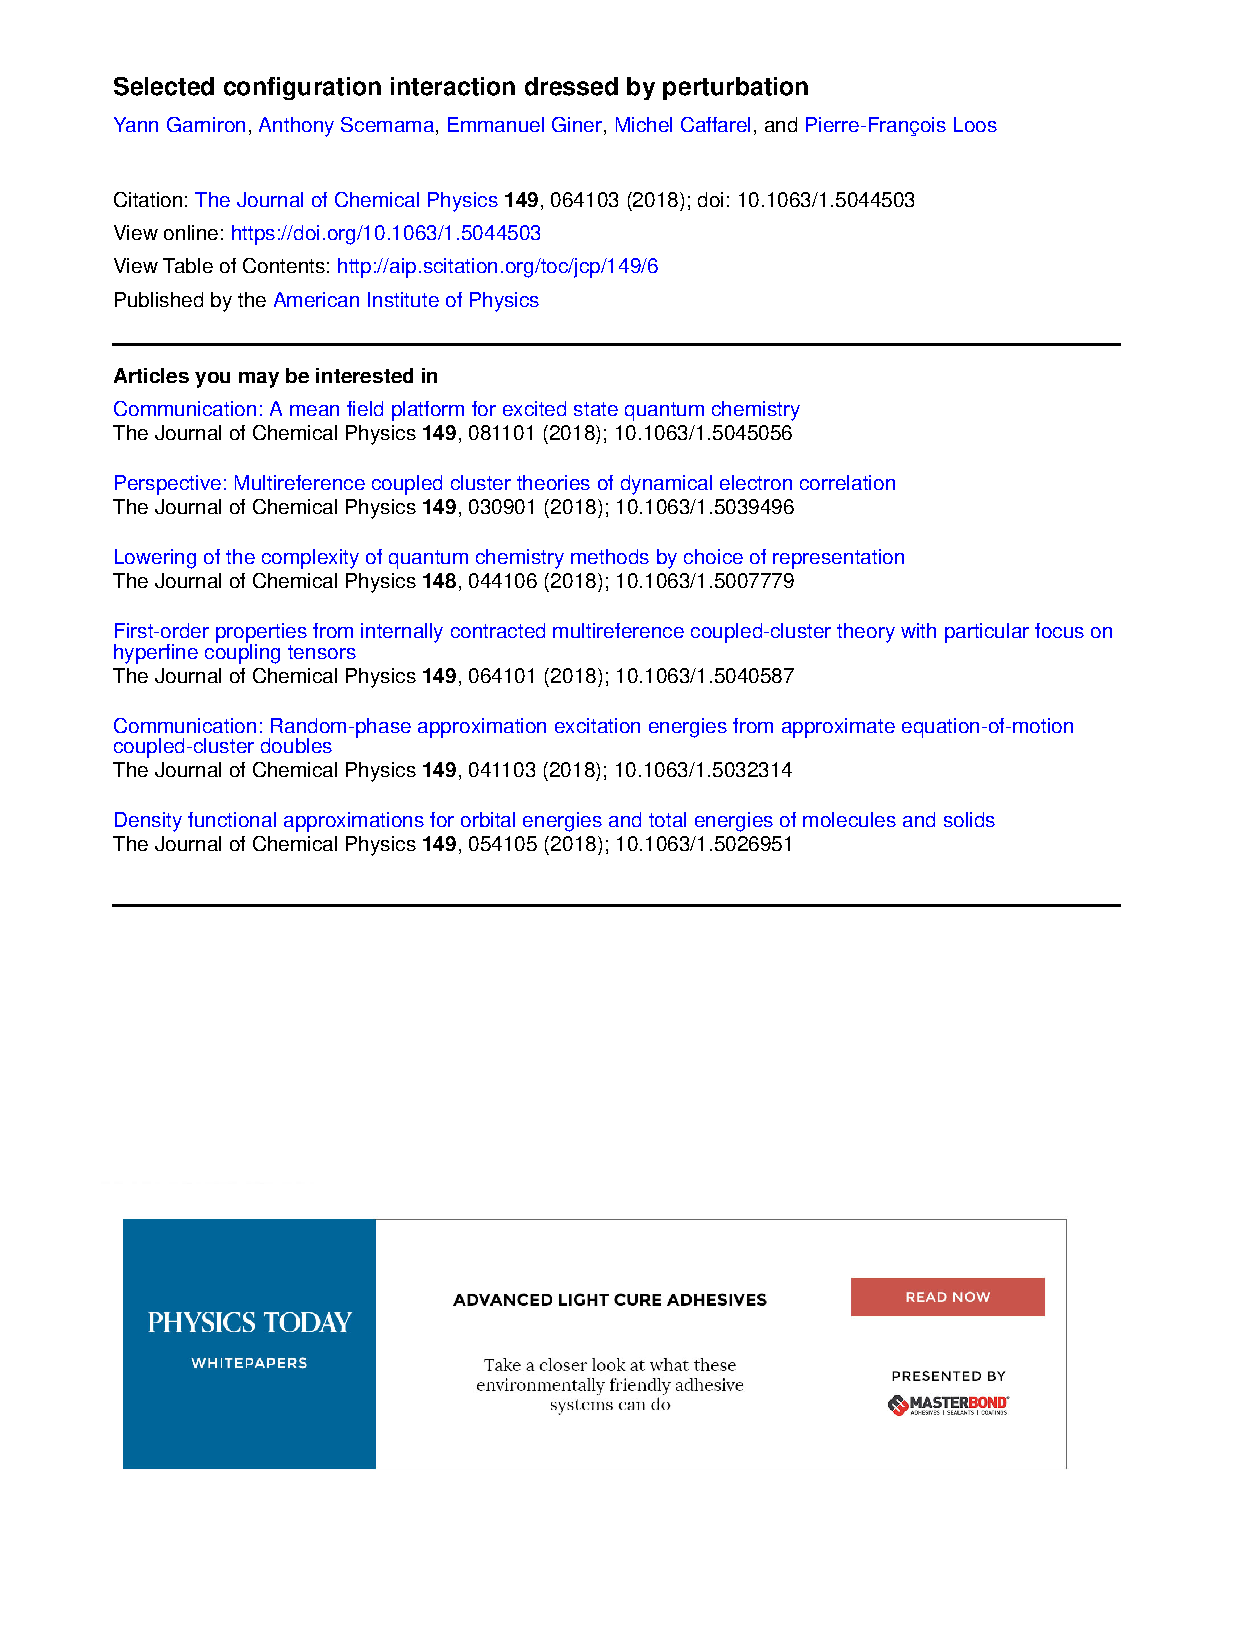
\includepdf[page=2-]{article_sbk}

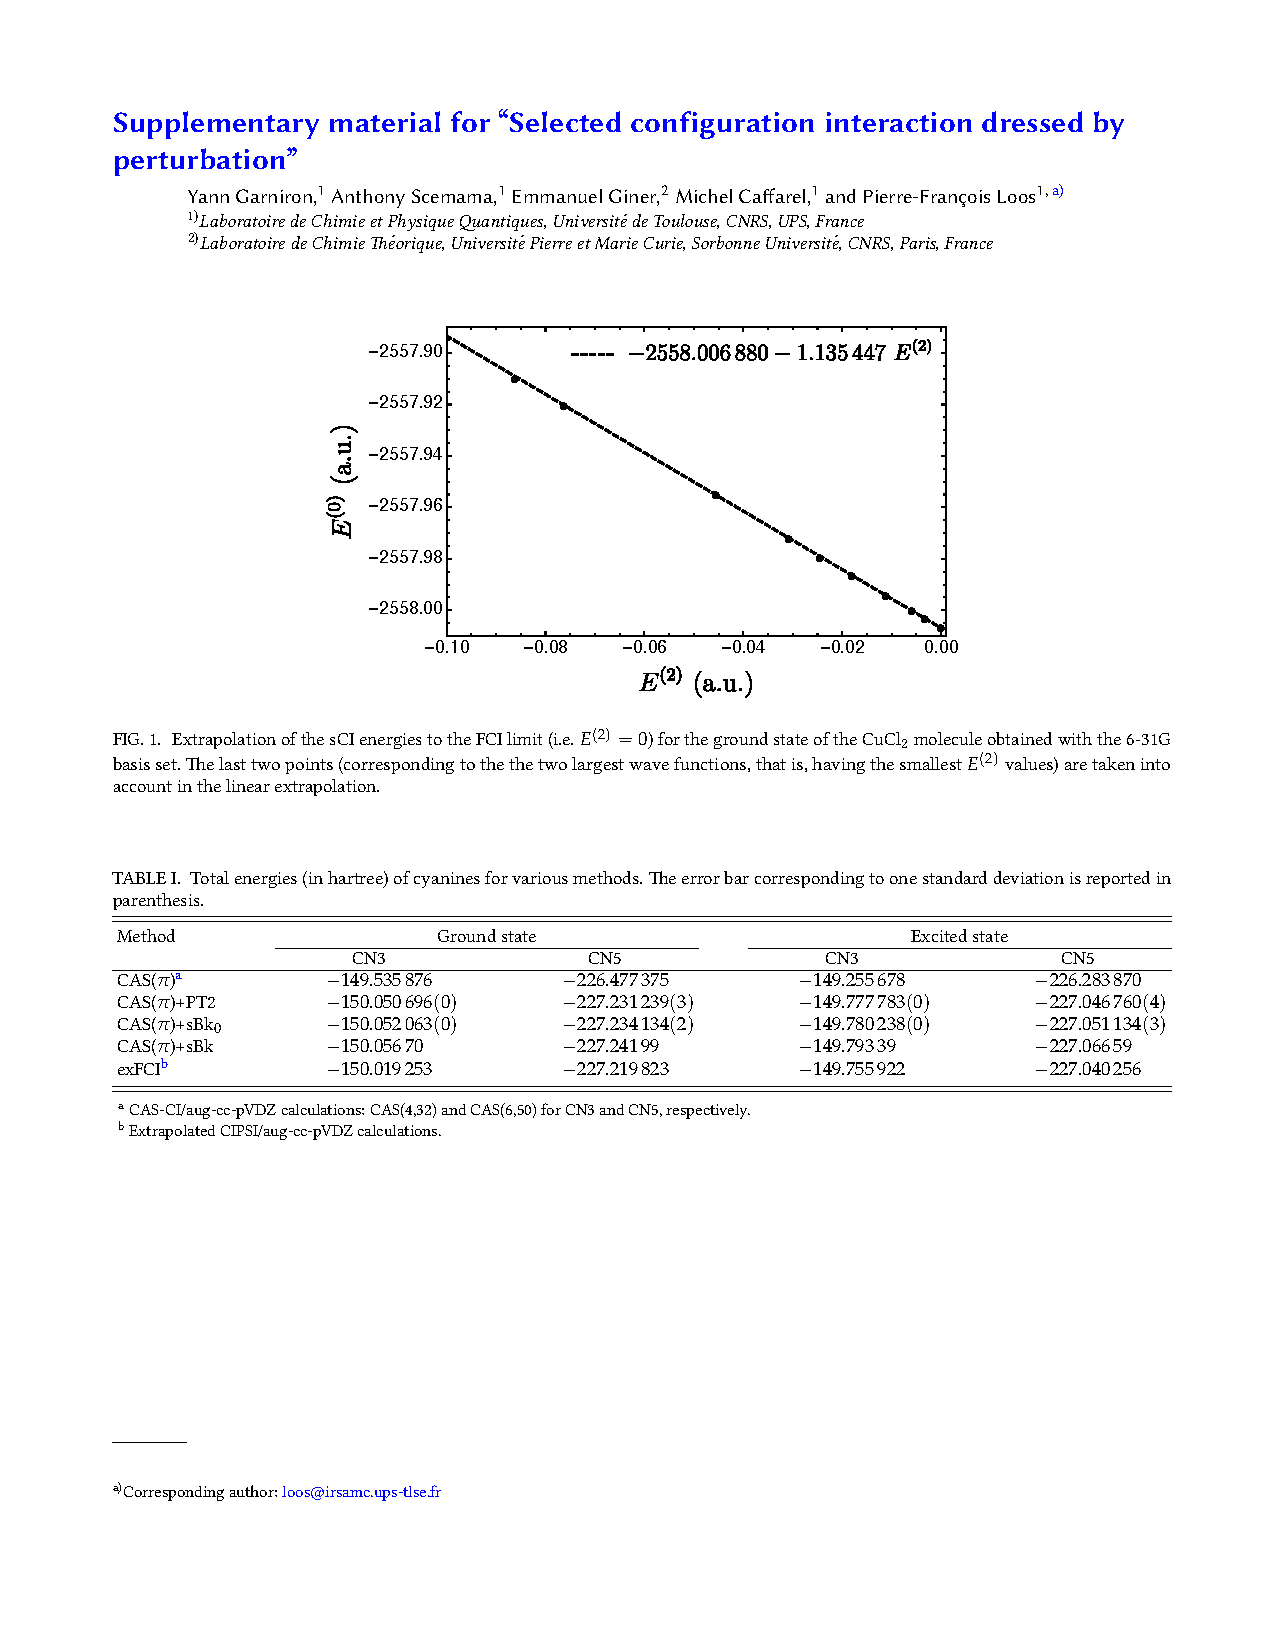
\includepdf[page=-]{article_sbk_sup}


\end{document}
